% Options for packages loaded elsewhere
\PassOptionsToPackage{unicode}{hyperref}
\PassOptionsToPackage{hyphens}{url}
%
\documentclass[
  letterpaper,
]{article}
\usepackage{amsmath,amssymb}
\usepackage{lmodern}
\usepackage{iftex}
\ifPDFTeX
  \usepackage[T1]{fontenc}
  \usepackage[utf8]{inputenc}
  \usepackage{textcomp} % provide euro and other symbols
\else % if luatex or xetex
  \usepackage{unicode-math}
  \defaultfontfeatures{Scale=MatchLowercase}
  \defaultfontfeatures[\rmfamily]{Ligatures=TeX,Scale=1}
\fi
% Use upquote if available, for straight quotes in verbatim environments
\IfFileExists{upquote.sty}{\usepackage{upquote}}{}
\IfFileExists{microtype.sty}{% use microtype if available
  \usepackage[]{microtype}
  \UseMicrotypeSet[protrusion]{basicmath} % disable protrusion for tt fonts
}{}
\makeatletter
\@ifundefined{KOMAClassName}{% if non-KOMA class
  \IfFileExists{parskip.sty}{%
    \usepackage{parskip}
  }{% else
    \setlength{\parindent}{0pt}
    \setlength{\parskip}{6pt plus 2pt minus 1pt}}
}{% if KOMA class
  \KOMAoptions{parskip=half}}
\makeatother
\usepackage{xcolor}
\usepackage[margin=1in]{geometry}
\usepackage{longtable,booktabs,array}
\usepackage{calc} % for calculating minipage widths
% Correct order of tables after \paragraph or \subparagraph
\usepackage{etoolbox}
\makeatletter
\patchcmd\longtable{\par}{\if@noskipsec\mbox{}\fi\par}{}{}
\makeatother
% Allow footnotes in longtable head/foot
\IfFileExists{footnotehyper.sty}{\usepackage{footnotehyper}}{\usepackage{footnote}}
\makesavenoteenv{longtable}
\usepackage{graphicx}
\makeatletter
\def\maxwidth{\ifdim\Gin@nat@width>\linewidth\linewidth\else\Gin@nat@width\fi}
\def\maxheight{\ifdim\Gin@nat@height>\textheight\textheight\else\Gin@nat@height\fi}
\makeatother
% Scale images if necessary, so that they will not overflow the page
% margins by default, and it is still possible to overwrite the defaults
% using explicit options in \includegraphics[width, height, ...]{}
\setkeys{Gin}{width=\maxwidth,height=\maxheight,keepaspectratio}
% Set default figure placement to htbp
\makeatletter
\def\fps@figure{htbp}
\makeatother
\setlength{\emergencystretch}{3em} % prevent overfull lines
\providecommand{\tightlist}{%
  \setlength{\itemsep}{0pt}\setlength{\parskip}{0pt}}
\setcounter{secnumdepth}{5}
\ifLuaTeX
\usepackage[bidi=basic]{babel}
\else
\usepackage[bidi=default]{babel}
\fi
\babelprovide[main,import]{english}
% get rid of language-specific shorthands (see #6817):
\let\LanguageShortHands\languageshorthands
\def\languageshorthands#1{}
\usepackage{booktabs}
\usepackage{longtable}
\usepackage{array}
\usepackage{multirow}
\usepackage{wrapfig}
\usepackage{float}
\usepackage{colortbl}
\usepackage{pdflscape}
\usepackage{tabu}
\usepackage{threeparttable}
\usepackage{threeparttablex}
\usepackage[normalem]{ulem}
\usepackage{makecell}
\usepackage{xcolor}
\ifLuaTeX
  \usepackage{selnolig}  % disable illegal ligatures
\fi
\IfFileExists{bookmark.sty}{\usepackage{bookmark}}{\usepackage{hyperref}}
\IfFileExists{xurl.sty}{\usepackage{xurl}}{} % add URL line breaks if available
\urlstyle{same} % disable monospaced font for URLs
\hypersetup{
  pdftitle={Description of model revisions to the base models for copper rockfish},
  pdfauthor={Chantel R. Wetzel (NWFSC), Melissa H. Monk (SWFSC), and Julia Coates (CDFW)},
  pdflang={en},
  hidelinks,
  pdfcreator={LaTeX via pandoc}}

\title{Description of model revisions to the base models for copper rockfish}
\author{Chantel R. Wetzel (NWFSC), Melissa H. Monk (SWFSC), and Julia Coates (CDFW)}
\date{}

\begin{document}
\maketitle

{
\setcounter{tocdepth}{2}
\tableofcontents
}
\hypertarget{overview}{%
\section{Overview}\label{overview}}

Since the release of the documents and the start of the STAR panel each of the sub-area models, north and south of Point Conception, for copper rockfish in California have had revisions to the model data. Each of these changes is described below and comparisons between the model as presented in the assessment documents and the revised base models are provide below in the \protect\hyperlink{figures}{Figures Section}.

\hypertarget{data-revisions}{%
\section{Data Revisions}\label{data-revisions}}

\hypertarget{cdfw-rov-survey-data}{%
\subsection{CDFW ROV Survey Data}\label{cdfw-rov-survey-data}}

Revised data for the CDFW ROV survey were provided to the STAT late on Thursday May 18th, 2023. It was determined that the line identifications for transects were not completely unique as previously thought. A small subset of transects were identified to have disparate sampling sites combined into transects (i.e., data collected across separate transects were combined into incorrect transects). This issue was identified to have occurred in a total of 24 out of the 1810 transects conducted statewide across all years. As a result the data within select transects were modified and 12 additional transects were added to the dataset. However, when the revised data were analyzed there were changes in the estimated index of abundance south of Point Conception greater than would be expected given the limited changes in the data described by CDFW. Upon further analysis of the data there were non-trivial revisions in estimates of varying attributes (e.g., proportion substrate type, depth, effort estimated through usable transect area) for 2019. The number of data points where measurements varied were greater than the number of transects with revisions. Additionally, south of Point Conception none of the newly identified transects occurred in 2019. The STAT communicated these unexpected findings to CDFW on May 24th, 2023.

Unfortunately, given the limited timing to properly review and analyze any potential data corrections, the STAT make the decision to remove the ROV data from both sub-area models. While the STAT only identified issues with the revised data south of Point Conception, there were overall concerns that all of the ROV data requires additional QA/QC to ensure that the data are accurate.

\hypertarget{recreational-removals-in-2020-and-2021}{%
\subsection{Recreational Removals in 2020 and 2021}\label{recreational-removals-in-2020-and-2021}}

CDFW communicated to the STAT that the 2020 and 2021 recreational catches for each sub-area appeared to be higher than expected. The recreational catches for these years were comprised of information from three sources do to sampling impacts related to COVID-19: copper rockfish sepeciated catches within RecFIN, CDFW generated proxy estimates for months with missing catches in 2020, and estimates of Sebastes genus catches in RecFIN that should be assigned as copper rockfish catches provided by CDFW. However, there was a miscommunication between the STAT and CDFW where the catch assigned to copper rockfish from the Sebastes genus also included the speciated catches for copper rockfish within RecFIN. Hence, adding the catches for copper rockfish within RecFIN resulted in a double counting of a subset of catches. On May 25th, 2023 CDFW provided revised Sebastes genus catches that did not include other copper rockfish RecFIN catches. The revised catches for the recreational CPFV and PR fleets in 2020 and 2021 decreased from the values in the original base model. The revised catches by fleet and year are:

\textbf{South of Point Conception}\\
2020: CPFV 43.42 mt and PR 19.71 mt\\
2021: CPFV 32.21 mt and no revisions to the PR catches

\textbf{North of Point Conception}\\
2020: CPFV 36.47 mt and PR 55.13 mt\\
2021: CPFV 31.91 mt and no revisions to the PR catches

\hypertarget{revised-base-models}{%
\subsection{Revised Base Models}\label{revised-base-models}}

These revisions to each sub-area base model resulted in very small changes in the model estimates. The California estimate of fraction unfished in 2023 change to 40.8 percent from 42.1 percent. The fraction of unfished spawning output in 2023 for the area south of Point Conception increased to 14.8 percent from 13.7 percent and the area north of Point Conception decreased to 51.9 percent from 53.9 percent. Comparisons of the estimated spawning output and fraction unfished for each sub-area are shown in Figures \ref{fig:south-ssb} - \ref{fig:north-depl}. Summaries of the combined California revised time series are shown in Table \ref{tab:ca-status} and new projections are shown in Table \ref{tab:ca-proj}. Time series estimates for each sub-area model are shown in Tables \ref{tab:tab-south-ts} and \ref{tab:tab-north-ts}.

\pagebreak

\hypertarget{tables}{%
\section{Tables}\label{tables}}

\hypertarget{california-stock}{%
\subsection{California Stock}\label{california-stock}}

\begingroup\fontsize{10}{12}\selectfont
\begingroup\fontsize{10}{12}\selectfont

\begin{longtable}[t]{c>{\centering\arraybackslash}p{1.83cm}>{\centering\arraybackslash}p{1.83cm}>{\centering\arraybackslash}p{1.83cm}>{\centering\arraybackslash}p{1.83cm}>{\centering\arraybackslash}p{1.83cm}}
\caption{\label{tab:ca-status}The estimated total biomass (mt), total biomass age 3+ (mt), age-0 recruits, and spawning ouput in number of billions of eggs across California and fraction unfished by year.}\\
\toprule
Year & Total Biomass (mt) & Total Biomass 3+ (mt) & Age-0 Recruits & Spawning Output & Fraction Unfished\\
\midrule
\endfirsthead
\caption[]{\label{tab:ca-status}The estimated total biomass (mt), total biomass age 3+ (mt), age-0 recruits, and spawning ouput in number of billions of eggs across California and fraction unfished by year. \textit{(continued)}}\\
\toprule
Year & Total Biomass (mt) & Total Biomass 3+ (mt) & Age-0 Recruits & Spawning Output & Fraction Unfished\\
\midrule
\endhead

\endfoot
\bottomrule
\endlastfoot
1916 & 6665.74 & 6621.52 & 482.15 & 678.06 & 1.001\\
1917 & 6663.58 & 6619.34 & 482.23 & 677.77 & 1.001\\
1918 & 6659.50 & 6615.23 & 482.31 & 677.25 & 1.000\\
1919 & 6654.70 & 6610.41 & 482.41 & 676.64 & 0.999\\
1920 & 6652.98 & 6608.66 & 482.52 & 676.36 & 0.999\\
1921 & 6651.54 & 6607.19 & 482.63 & 676.10 & 0.999\\
1922 & 6651.26 & 6606.88 & 482.76 & 675.97 & 0.998\\
1923 & 6651.97 & 6607.56 & 482.90 & 675.95 & 0.998\\
1924 & 6652.85 & 6608.39 & 483.05 & 675.95 & 0.998\\
1925 & 6655.31 & 6610.81 & 483.21 & 676.12 & 0.999\\
1926 & 6656.86 & 6612.32 & 483.39 & 676.19 & 0.999\\
1927 & 6657.75 & 6613.16 & 483.58 & 676.18 & 0.999\\
1928 & 6660.32 & 6615.67 & 483.79 & 676.35 & 0.999\\
1929 & 6661.70 & 6616.98 & 484.03 & 676.40 & 0.999\\
1930 & 6662.49 & 6617.71 & 484.28 & 676.39 & 0.999\\
1931 & 6661.09 & 6616.22 & 484.55 & 676.11 & 0.999\\
1932 & 6658.22 & 6613.27 & 484.85 & 675.66 & 0.998\\
1933 & 6655.47 & 6610.44 & 485.18 & 675.20 & 0.997\\
1934 & 6653.34 & 6608.21 & 485.53 & 674.79 & 0.997\\
1935 & 6652.12 & 6606.88 & 485.92 & 674.46 & 0.996\\
1936 & 6648.41 & 6603.05 & 486.33 & 673.83 & 0.995\\
1937 & 6645.32 & 6599.83 & 486.78 & 673.24 & 0.994\\
1938 & 6640.19 & 6594.56 & 487.25 & 672.41 & 0.993\\
1939 & 6637.87 & 6592.09 & 487.78 & 671.84 & 0.992\\
1940 & 6639.21 & 6593.28 & 488.36 & 671.63 & 0.992\\
1941 & 6637.36 & 6591.23 & 488.98 & 671.07 & 0.991\\
1942 & 6638.07 & 6591.73 & 489.65 & 670.74 & 0.991\\
1943 & 6651.32 & 6604.75 & 490.38 & 671.70 & 0.992\\
1944 & 6665.47 & 6618.63 & 491.15 & 672.74 & 0.994\\
1945 & 6677.39 & 6630.24 & 491.98 & 673.48 & 0.995\\
1946 & 6677.19 & 6629.70 & 492.85 & 672.82 & 0.994\\
1947 & 6671.49 & 6623.65 & 493.74 & 671.53 & 0.992\\
1948 & 6687.43 & 6639.24 & 494.63 & 672.55 & 0.993\\
1949 & 6691.40 & 6642.88 & 495.47 & 672.32 & 0.993\\
1950 & 6695.42 & 6646.58 & 496.26 & 672.09 & 0.993\\
1951 & 6696.37 & 6647.26 & 496.98 & 671.52 & 0.992\\
1952 & 6683.57 & 6634.26 & 497.53 & 669.45 & 0.989\\
1953 & 6684.32 & 6634.87 & 497.96 & 668.76 & 0.988\\
1954 & 6697.10 & 6647.53 & 498.14 & 669.37 & 0.989\\
1955 & 6697.13 & 6647.40 & 497.83 & 668.81 & 0.988\\
1956 & 6685.26 & 6635.33 & 497.13 & 667.23 & 0.985\\
1957 & 6666.31 & 6616.15 & 496.23 & 664.91 & 0.982\\
1958 & 6659.72 & 6609.34 & 495.74 & 663.68 & 0.980\\
1959 & 6614.59 & 6564.32 & 495.87 & 658.57 & 0.973\\
1960 & 6597.06 & 6546.78 & 497.66 & 656.06 & 0.969\\
1961 & 6594.01 & 6543.42 & 500.69 & 654.98 & 0.967\\
1962 & 6608.70 & 6557.09 & 505.05 & 655.75 & 0.969\\
1963 & 6617.96 & 6564.48 & 512.55 & 655.94 & 0.969\\
1964 & 6617.16 & 6561.32 & 527.12 & 654.78 & 0.967\\
1965 & 6629.54 & 6571.11 & 558.21 & 654.29 & 0.966\\
1966 & 6615.31 & 6552.65 & 615.24 & 650.22 & 0.960\\
1967 & 6577.04 & 6508.29 & 695.86 & 642.63 & 0.949\\
1968 & 6551.00 & 6477.15 & 746.84 & 634.60 & 0.937\\
1969 & 6539.19 & 6464.98 & 635.85 & 626.61 & 0.925\\
1970 & 6557.60 & 6489.67 & 526.09 & 621.21 & 0.918\\
1971 & 6530.29 & 6474.56 & 457.53 & 613.60 & 0.906\\
1972 & 6510.29 & 6464.63 & 538.17 & 610.85 & 0.902\\
1973 & 6390.17 & 6352.34 & 586.87 & 604.03 & 0.892\\
1974 & 6177.83 & 6140.77 & 472.92 & 592.43 & 0.875\\
1975 & 5870.72 & 5832.79 & 412.89 & 572.93 & 0.846\\
1976 & 5524.48 & 5490.98 & 405.92 & 548.26 & 0.810\\
1977 & 5147.29 & 5115.36 & 455.86 & 517.75 & 0.765\\
1978 & 4749.06 & 4718.55 & 402.57 & 482.50 & 0.713\\
1979 & 4364.90 & 4335.09 & 320.29 & 446.47 & 0.659\\
1980 & 3917.41 & 3892.59 & 279.21 & 402.84 & 0.595\\
1981 & 3458.40 & 3437.45 & 294.28 & 356.56 & 0.527\\
1982 & 3078.58 & 3056.57 & 269.48 & 317.46 & 0.469\\
1983 & 2633.89 & 2608.33 & 243.21 & 272.41 & 0.402\\
1984 & 2353.60 & 2332.26 & 291.47 & 241.25 & 0.356\\
1985 & 2103.04 & 2079.73 & 419.48 & 212.66 & 0.314\\
1986 & 1824.01 & 1790.04 & 373.92 & 180.96 & 0.267\\
1987 & 1626.73 & 1588.78 & 319.50 & 156.06 & 0.230\\
1988 & 1547.81 & 1520.37 & 321.68 & 141.31 & 0.209\\
1989 & 1504.22 & 1479.34 & 304.37 & 130.30 & 0.192\\
1990 & 1462.66 & 1435.48 & 362.01 & 121.79 & 0.180\\
1991 & 1412.03 & 1379.44 & 389.95 & 115.07 & 0.170\\
1992 & 1380.73 & 1345.35 & 275.27 & 110.19 & 0.163\\
1993 & 1371.96 & 1342.39 & 182.87 & 106.30 & 0.157\\
1994 & 1365.02 & 1339.74 & 178.23 & 102.74 & 0.152\\
1995 & 1382.39 & 1355.93 & 206.70 & 103.77 & 0.153\\
1996 & 1426.53 & 1404.58 & 160.52 & 107.69 & 0.159\\
1997 & 1408.55 & 1389.81 & 129.14 & 108.00 & 0.160\\
1998 & 1438.06 & 1419.55 & 159.86 & 112.18 & 0.166\\
1999 & 1479.02 & 1459.39 & 354.14 & 118.48 & 0.175\\
2000 & 1521.72 & 1499.53 & 180.90 & 125.66 & 0.186\\
2001 & 1587.07 & 1562.39 & 122.55 & 133.94 & 0.198\\
2002 & 1659.47 & 1641.63 & 206.82 & 141.99 & 0.210\\
2003 & 1739.64 & 1721.65 & 347.14 & 150.73 & 0.223\\
2004 & 1807.71 & 1785.57 & 159.37 & 159.23 & 0.235\\
2005 & 1876.31 & 1853.48 & 233.65 & 167.79 & 0.248\\
2006 & 1908.80 & 1892.41 & 87.13 & 172.99 & 0.255\\
2007 & 1948.26 & 1929.63 & 327.83 & 178.43 & 0.264\\
2008 & 1959.04 & 1932.92 & 316.70 & 181.36 & 0.268\\
2009 & 1995.05 & 1945.34 & 855.92 & 184.79 & 0.273\\
2010 & 2058.62 & 2011.30 & 916.09 & 186.60 & 0.276\\
2011 & 2181.60 & 2118.59 & 408.40 & 189.28 & 0.280\\
2012 & 2332.58 & 2285.44 & 549.63 & 192.55 & 0.284\\
2013 & 2496.77 & 2459.04 & 899.07 & 199.52 & 0.295\\
2014 & 2652.33 & 2599.55 & 238.58 & 211.72 & 0.313\\
2015 & 2817.45 & 2764.38 & 99.08 & 228.19 & 0.337\\
2016 & 2927.78 & 2896.95 & 241.39 & 241.80 & 0.357\\
2017 & 2997.80 & 2967.85 & 126.19 & 253.20 & 0.374\\
2018 & 2983.01 & 2955.28 & 93.44 & 257.10 & 0.380\\
2019 & 2963.64 & 2921.29 & 104.42 & 260.98 & 0.385\\
2020 & 2953.56 & 2923.62 & 167.39 & 263.49 & 0.389\\
2021 & 2943.40 & 2920.84 & 319.75 & 264.13 & 0.390\\
2022 & 2968.49 & 2937.35 & 310.70 & 267.42 & 0.395\\
2023 & 3052.60 & 3017.07 & 308.64 & 276.58 & 0.409\\*
\end{longtable}
\endgroup{}
\endgroup{}

\newpage

\begingroup\fontsize{10}{12}\selectfont

\begin{landscape}\begingroup\fontsize{10}{12}\selectfont

\begin{longtable}[t]{c>{\centering\arraybackslash}p{1.5cm}>{\centering\arraybackslash}p{1.5cm}>{\centering\arraybackslash}p{1.5cm}>{\centering\arraybackslash}p{1.5cm}>{\centering\arraybackslash}p{1.5cm}>{\centering\arraybackslash}p{1.5cm}>{\centering\arraybackslash}p{1.5cm}c}
\caption{\label{tab:ca-proj}The estimated OFL, ABC, buffer, spawning output in billions of eggs across California, and relative spawning outut by year.}\\
\toprule
Year & Adopted OFL (mt) & Adopted ACL (mt) & Assumed Catch (mt) & OFL (mt) & ABC (mt) & Buffer & Spawning Output & Relative Spawning Ouptut\\
\midrule
\endfirsthead
\caption[]{\label{tab:ca-proj}The estimated OFL, ABC, buffer, spawning output in billions of eggs across California, and relative spawning outut by year. \textit{(continued)}}\\
\toprule
Year & Adopted OFL (mt) & Adopted ACL (mt) & Assumed Catch (mt) & OFL (mt) & ABC (mt) & Buffer & Spawning Output & Relative Spawning Ouptut\\
\midrule
\endhead

\endfoot
\bottomrule
\endlastfoot
2023 & 116.4 & 91.5 & 91.53 & - & - & - & 276.58 & 0.408\\
2024 & 121.3 & 94.7 & 94.69 & - & - & - & 283.63 & 0.419\\
2025 & - & - & - & 164.2 & 153.6 & 0.935 & 289.99 & 0.428\\
2026 & - & - & - & 164.4 & 152.9 & 0.93 & 290.48 & 0.429\\
2027 & - & - & - & 164.5 & 152.4 & 0.926 & 290.61 & 0.429\\
2028 & - & - & - & 164.5 & 151.6 & 0.922 & 290.55 & 0.429\\
2029 & - & - & - & 164.3 & 150.7 & 0.917 & 290.39 & 0.429\\
2030 & - & - & - & 164.1 & 149.8 & 0.913 & 290.21 & 0.429\\
2031 & - & - & - & 163.9 & 149 & 0.909 & 290.05 & 0.428\\
2032 & - & - & - & 163.7 & 148 & 0.904 & 289.91 & 0.428\\
2033 & - & - & - & 163.6 & 147.3 & 0.9 & 289.84 & 0.428\\
2034 & - & - & - & 163.6 & 146.6 & 0.896 & 289.84 & 0.428\\*
\end{longtable}
\endgroup{}
\end{landscape}
\endgroup{}

\newpage

\hypertarget{south-of-point-conception}{%
\subsection{South of Point Conception}\label{south-of-point-conception}}

\begingroup\fontsize{10}{12}\selectfont
\begingroup\fontsize{10}{12}\selectfont

\begin{longtable}[t]{l>{\raggedright\arraybackslash}p{1.22cm}>{\raggedright\arraybackslash}p{1.22cm}>{\raggedright\arraybackslash}p{1.22cm}>{\raggedright\arraybackslash}p{1.22cm}>{\raggedright\arraybackslash}p{1.22cm}>{\raggedright\arraybackslash}p{1.22cm}>{\raggedright\arraybackslash}p{1.22cm}>{\raggedright\arraybackslash}p{1.22cm}}
\caption{\label{tab:tab-south-ts}Time series of population estimates from the revised base model for the sub-area south of Point Conception.}\\
\toprule
Year & Total Biomass (mt) & Spawning Output & Total Biomass 3+ (mt) & Fraction Unfished & Age-0 Recruits & Total Mortality (mt) & 1-SPR & Exploitation Rate\\
\midrule
\endfirsthead
\caption[]{\label{tab:tab-south-ts}Time series of population estimates from the revised base model for the sub-area south of Point Conception. \textit{(continued)}}\\
\toprule
Year & Total Biomass (mt) & Spawning Output & Total Biomass 3+ (mt) & Fraction Unfished & Age-0 Recruits & Total Mortality (mt) & 1-SPR & Exploitation Rate\\
\midrule
\endhead

\endfoot
\bottomrule
\endlastfoot
1916 & 2011.020 & 201.659 & 1993.320 & 1.000 & 241.073 & 0.120 & 0.001 & 0.000\\
1917 & 2011.030 & 201.657 & 1993.330 & 1.000 & 241.113 & 0.195 & 0.001 & 0.000\\
1918 & 2010.980 & 201.648 & 1993.270 & 1.000 & 241.157 & 0.177 & 0.001 & 0.000\\
1919 & 2010.970 & 201.642 & 1993.260 & 1.000 & 241.204 & 0.106 & 0.001 & 0.000\\
1920 & 2011.050 & 201.646 & 1993.340 & 1.000 & 241.258 & 0.115 & 0.001 & 0.000\\
1921 & 2011.150 & 201.651 & 1993.430 & 1.000 & 241.315 & 0.101 & 0.001 & 0.000\\
1922 & 2011.280 & 201.660 & 1993.560 & 1.000 & 241.379 & 0.099 & 0.001 & 0.000\\
1923 & 2011.430 & 201.671 & 1993.710 & 1.001 & 241.448 & 0.132 & 0.001 & 0.000\\
1924 & 2011.580 & 201.681 & 1993.850 & 1.001 & 241.523 & 0.178 & 0.001 & 0.000\\
1925 & 2011.700 & 201.688 & 1993.970 & 1.001 & 241.605 & 0.195 & 0.001 & 0.000\\
1926 & 2011.840 & 201.696 & 1994.100 & 1.001 & 241.694 & 0.242 & 0.002 & 0.000\\
1927 & 2011.960 & 201.702 & 1994.220 & 1.001 & 241.791 & 0.201 & 0.001 & 0.000\\
1928 & 2012.160 & 201.715 & 1994.410 & 1.001 & 241.897 & 0.201 & 0.001 & 0.000\\
1929 & 2012.390 & 201.731 & 1994.630 & 1.001 & 242.013 & 0.223 & 0.002 & 0.000\\
1930 & 2012.630 & 201.748 & 1994.860 & 1.001 & 242.140 & 0.256 & 0.002 & 0.000\\
1931 & 2012.870 & 201.766 & 1995.090 & 1.001 & 242.277 & 0.253 & 0.002 & 0.000\\
1932 & 2013.160 & 201.787 & 1995.370 & 1.001 & 242.426 & 0.335 & 0.002 & 0.000\\
1933 & 2013.400 & 201.803 & 1995.610 & 1.001 & 242.588 & 0.206 & 0.002 & 0.000\\
1934 & 2013.820 & 201.836 & 1996.010 & 1.001 & 242.767 & 0.302 & 0.002 & 0.000\\
1935 & 2014.190 & 201.864 & 1996.370 & 1.002 & 242.959 & 0.596 & 0.004 & 0.000\\
1936 & 2014.330 & 201.866 & 1996.500 & 1.002 & 243.165 & 0.437 & 0.003 & 0.000\\
1937 & 2014.700 & 201.889 & 1996.850 & 1.002 & 243.390 & 1.186 & 0.008 & 0.001\\
1938 & 2014.420 & 201.841 & 1996.550 & 1.001 & 243.627 & 0.707 & 0.005 & 0.000\\
1939 & 2014.700 & 201.852 & 1996.820 & 1.001 & 243.890 & 0.491 & 0.004 & 0.000\\
1940 & 2015.290 & 201.893 & 1997.400 & 1.002 & 244.179 & 0.533 & 0.004 & 0.000\\
1941 & 2015.950 & 201.938 & 1998.030 & 1.002 & 244.491 & 0.591 & 0.004 & 0.000\\
1942 & 2016.650 & 201.987 & 1998.710 & 1.002 & 244.825 & 0.138 & 0.001 & 0.000\\
1943 & 2017.910 & 202.093 & 1999.950 & 1.003 & 245.190 & 0.199 & 0.001 & 0.000\\
1944 & 2019.210 & 202.202 & 2001.220 & 1.003 & 245.577 & 0.082 & 0.001 & 0.000\\
1945 & 2020.720 & 202.334 & 2002.700 & 1.004 & 245.990 & 0.162 & 0.001 & 0.000\\
1946 & 2022.260 & 202.467 & 2004.210 & 1.004 & 246.423 & 0.199 & 0.002 & 0.000\\
1947 & 2023.860 & 202.607 & 2005.780 & 1.005 & 246.870 & 0.742 & 0.006 & 0.000\\
1948 & 2025.000 & 202.704 & 2006.890 & 1.006 & 247.314 & 1.783 & 0.015 & 0.001\\
1949 & 2025.160 & 202.709 & 2007.020 & 1.006 & 247.737 & 2.323 & 0.019 & 0.001\\
1950 & 2024.890 & 202.665 & 2006.720 & 1.005 & 248.132 & 3.154 & 0.026 & 0.002\\
1951 & 2023.920 & 202.546 & 2005.710 & 1.005 & 248.488 & 5.837 & 0.042 & 0.003\\
1952 & 2020.630 & 202.149 & 2002.400 & 1.003 & 248.764 & 4.472 & 0.034 & 0.002\\
1953 & 2018.950 & 201.929 & 2000.700 & 1.002 & 248.982 & 4.126 & 0.033 & 0.002\\
1954 & 2017.830 & 201.776 & 1999.560 & 1.001 & 249.069 & 8.557 & 0.069 & 0.004\\
1955 & 2012.280 & 201.222 & 1993.990 & 0.998 & 248.917 & 16.723 & 0.131 & 0.008\\
1956 & 1998.340 & 199.885 & 1980.050 & 0.992 & 248.567 & 18.308 & 0.143 & 0.009\\
1957 & 1982.950 & 198.360 & 1964.680 & 0.984 & 248.113 & 10.817 & 0.088 & 0.006\\
1958 & 1975.840 & 197.535 & 1957.590 & 0.980 & 247.868 & 10.863 & 0.088 & 0.006\\
1959 & 1969.310 & 196.756 & 1951.090 & 0.976 & 247.937 & 5.910 & 0.049 & 0.003\\
1960 & 1968.510 & 196.525 & 1950.300 & 0.975 & 248.829 & 6.771 & 0.055 & 0.003\\
1961 & 1967.360 & 196.301 & 1949.140 & 0.974 & 250.347 & 9.631 & 0.075 & 0.005\\
1962 & 1963.840 & 195.862 & 1945.540 & 0.972 & 252.525 & 6.549 & 0.052 & 0.003\\
1963 & 1963.990 & 195.781 & 1945.560 & 0.971 & 256.273 & 6.984 & 0.056 & 0.004\\
1964 & 1964.300 & 195.711 & 1945.680 & 0.971 & 263.561 & 11.763 & 0.095 & 0.006\\
1965 & 1960.390 & 195.231 & 1941.430 & 0.969 & 279.106 & 17.350 & 0.136 & 0.009\\
1966 & 1951.960 & 194.232 & 1932.320 & 0.964 & 307.619 & 43.743 & 0.308 & 0.023\\
1967 & 1918.280 & 190.733 & 1897.270 & 0.946 & 347.931 & 50.617 & 0.350 & 0.027\\
1968 & 1881.810 & 186.516 & 1858.540 & 0.925 & 373.421 & 59.242 & 0.403 & 0.032\\
1969 & 1843.520 & 181.572 & 1817.640 & 0.901 & 317.927 & 46.966 & 0.343 & 0.026\\
1970 & 1827.080 & 178.091 & 1800.620 & 0.884 & 263.045 & 69.547 & 0.459 & 0.039\\
1971 & 1794.900 & 173.227 & 1772.480 & 0.859 & 228.766 & 66.829 & 0.446 & 0.038\\
1972 & 1768.240 & 169.521 & 1749.420 & 0.841 & 269.084 & 92.190 & 0.552 & 0.053\\
1973 & 1713.140 & 164.475 & 1695.670 & 0.816 & 293.433 & 111.467 & 0.627 & 0.066\\
1974 & 1633.520 & 157.923 & 1613.450 & 0.784 & 236.458 & 138.129 & 0.719 & 0.086\\
1975 & 1522.840 & 148.312 & 1502.260 & 0.736 & 206.447 & 142.100 & 0.756 & 0.095\\
1976 & 1406.430 & 137.353 & 1389.560 & 0.681 & 202.962 & 116.877 & 0.719 & 0.084\\
1977 & 1315.080 & 128.283 & 1299.950 & 0.636 & 227.931 & 108.991 & 0.717 & 0.084\\
1978 & 1230.650 & 120.043 & 1215.380 & 0.596 & 201.286 & 107.974 & 0.734 & 0.089\\
1979 & 1146.460 & 111.922 & 1130.210 & 0.555 & 160.147 & 151.669 & 0.854 & 0.134\\
1980 & 1016.540 & 99.538 & 1002.450 & 0.494 & 139.604 & 147.880 & 0.879 & 0.148\\
1981 & 889.274 & 87.101 & 877.839 & 0.432 & 147.141 & 85.595 & 0.760 & 0.098\\
1982 & 825.100 & 80.301 & 814.751 & 0.398 & 134.740 & 156.681 & 0.924 & 0.192\\
1983 & 686.222 & 67.335 & 675.650 & 0.334 & 121.607 & 82.038 & 0.823 & 0.121\\
1984 & 622.316 & 60.748 & 612.606 & 0.301 & 145.735 & 91.400 & 0.875 & 0.149\\
1985 & 549.667 & 53.389 & 540.272 & 0.265 & 209.740 & 115.712 & 0.941 & 0.214\\
1986 & 453.985 & 43.820 & 442.300 & 0.217 & 186.961 & 101.222 & 0.948 & 0.229\\
1987 & 377.910 & 35.425 & 362.935 & 0.176 & 159.750 & 78.315 & 0.937 & 0.216\\
1988 & 333.073 & 29.379 & 319.797 & 0.146 & 160.840 & 52.217 & 0.872 & 0.163\\
1989 & 322.046 & 26.315 & 310.322 & 0.131 & 152.187 & 53.416 & 0.868 & 0.172\\
1990 & 314.568 & 24.355 & 302.873 & 0.121 & 181.004 & 60.045 & 0.888 & 0.198\\
1991 & 302.255 & 22.761 & 290.612 & 0.113 & 194.975 & 52.570 & 0.856 & 0.181\\
1992 & 299.232 & 21.865 & 285.805 & 0.108 & 137.633 & 33.831 & 0.728 & 0.118\\
1993 & 318.055 & 22.724 & 304.725 & 0.113 & 91.434 & 19.979 & 0.524 & 0.066\\
1994 & 353.821 & 25.087 & 344.459 & 0.124 & 89.114 & 62.474 & 0.845 & 0.181\\
1995 & 344.693 & 24.978 & 338.002 & 0.124 & 103.350 & 51.232 & 0.786 & 0.152\\
1996 & 341.635 & 25.317 & 334.895 & 0.126 & 80.262 & 97.058 & 0.929 & 0.290\\
1997 & 284.965 & 21.882 & 277.779 & 0.109 & 64.568 & 42.804 & 0.777 & 0.154\\
1998 & 277.503 & 21.584 & 271.840 & 0.107 & 79.931 & 54.841 & 0.862 & 0.202\\
1999 & 254.073 & 20.041 & 248.958 & 0.099 & 177.070 & 49.755 & 0.886 & 0.200\\
2000 & 231.045 & 18.663 & 223.745 & 0.093 & 90.450 & 27.500 & 0.753 & 0.123\\
2001 & 231.013 & 18.565 & 219.439 & 0.092 & 61.274 & 20.500 & 0.666 & 0.093\\
2002 & 241.539 & 18.858 & 235.308 & 0.094 & 103.411 & 14.404 & 0.525 & 0.061\\
2003 & 260.446 & 19.867 & 255.178 & 0.099 & 173.568 & 17.502 & 0.540 & 0.069\\
2004 & 277.106 & 21.305 & 268.514 & 0.106 & 79.687 & 16.765 & 0.516 & 0.062\\
2005 & 296.113 & 23.028 & 284.825 & 0.114 & 116.826 & 29.840 & 0.699 & 0.105\\
2006 & 303.226 & 23.709 & 296.882 & 0.118 & 43.564 & 13.691 & 0.427 & 0.046\\
2007 & 326.301 & 25.635 & 318.736 & 0.127 & 163.915 & 32.282 & 0.691 & 0.101\\
2008 & 328.981 & 26.365 & 323.863 & 0.131 & 158.351 & 26.868 & 0.628 & 0.083\\
2009 & 336.126 & 27.429 & 323.823 & 0.136 & 427.960 & 24.856 & 0.602 & 0.077\\
2010 & 351.602 & 28.399 & 335.619 & 0.141 & 458.043 & 23.379 & 0.577 & 0.070\\
2011 & 384.634 & 29.304 & 353.078 & 0.145 & 204.199 & 44.786 & 0.771 & 0.127\\
2012 & 418.943 & 28.838 & 389.313 & 0.143 & 274.813 & 51.040 & 0.769 & 0.131\\
2013 & 465.228 & 29.218 & 448.883 & 0.145 & 449.535 & 79.539 & 0.841 & 0.177\\
2014 & 490.599 & 30.048 & 468.089 & 0.149 & 119.289 & 61.709 & 0.737 & 0.132\\
2015 & 534.564 & 33.464 & 506.967 & 0.166 & 49.538 & 82.178 & 0.798 & 0.162\\
2016 & 554.720 & 36.131 & 546.993 & 0.179 & 120.694 & 98.951 & 0.838 & 0.181\\
2017 & 541.435 & 37.560 & 536.740 & 0.186 & 63.095 & 86.863 & 0.809 & 0.162\\
2018 & 517.920 & 39.226 & 510.013 & 0.195 & 46.720 & 101.308 & 0.872 & 0.199\\
2019 & 459.119 & 37.922 & 454.749 & 0.188 & 52.210 & 80.702 & 0.861 & 0.177\\
2020 & 405.470 & 35.688 & 401.914 & 0.177 & 83.695 & 70.261 & 0.870 & 0.175\\
2021 & 352.528 & 32.447 & 348.093 & 0.161 & 159.874 & 45.165 & 0.805 & 0.130\\
2022 & 321.900 & 30.239 & 314.546 & 0.150 & 155.352 & 19.520 & 0.578 & 0.062\\
2023 & 320.717 & 29.760 & 309.056 & 0.148 & 154.319 & 26.800 & 0.696 & 0.087\\
2024 & 319.127 & 28.370 & 307.748 & 0.141 & 151.211 & 27.700 & 0.704 & 0.090\\
2025 & 324.527 & 27.199 & 313.256 & 0.135 & 148.456 & 44.530 & 0.829 & 0.142\\
2026 & 319.071 & 25.451 & 308.030 & 0.126 & 144.091 & 44.340 & 0.819 & 0.144\\
2027 & 317.052 & 24.464 & 306.236 & 0.121 & 141.479 & 44.190 & 0.810 & 0.144\\
2028 & 316.863 & 24.010 & 306.337 & 0.119 & 140.239 & 43.970 & 0.801 & 0.144\\
2029 & 317.581 & 23.882 & 307.223 & 0.118 & 139.886 & 43.700 & 0.795 & 0.142\\
2030 & 318.703 & 23.936 & 308.421 & 0.119 & 140.034 & 43.440 & 0.790 & 0.141\\
2031 & 319.983 & 24.072 & 309.719 & 0.119 & 140.412 & 43.210 & 0.787 & 0.140\\
2032 & 321.349 & 24.235 & 311.069 & 0.120 & 140.858 & 42.920 & 0.783 & 0.138\\
2033 & 322.916 & 24.407 & 312.608 & 0.121 & 141.325 & 42.710 & 0.781 & 0.137\\
2034 & 324.686 & 24.582 & 314.344 & 0.122 & 141.797 & 42.510 & 0.778 & 0.135\\*
\end{longtable}
\endgroup{}
\endgroup{}

\newpage

\hypertarget{north-of-point-conception}{%
\subsection{North of Point Conception}\label{north-of-point-conception}}

\begingroup\fontsize{10}{12}\selectfont
\begingroup\fontsize{10}{12}\selectfont

\begin{longtable}[t]{l>{\raggedright\arraybackslash}p{1.22cm}>{\raggedright\arraybackslash}p{1.22cm}>{\raggedright\arraybackslash}p{1.22cm}>{\raggedright\arraybackslash}p{1.22cm}>{\raggedright\arraybackslash}p{1.22cm}>{\raggedright\arraybackslash}p{1.22cm}>{\raggedright\arraybackslash}p{1.22cm}>{\raggedright\arraybackslash}p{1.22cm}}
\caption{\label{tab:tab-north-ts}Time series of population estimates from the revised base model for the sub-area north of Point Conception.}\\
\toprule
Year & Total Biomass (mt) & Spawning Output & Total Biomass 3+ (mt) & Fraction Unfished & Age-0 Recruits & Total Mortality (mt) & 1-SPR & Exploitation Rate\\
\midrule
\endfirsthead
\caption[]{\label{tab:tab-north-ts}Time series of population estimates from the revised base model for the sub-area north of Point Conception. \textit{(continued)}}\\
\toprule
Year & Total Biomass (mt) & Spawning Output & Total Biomass 3+ (mt) & Fraction Unfished & Age-0 Recruits & Total Mortality (mt) & 1-SPR & Exploitation Rate\\
\midrule
\endhead

\endfoot
\bottomrule
\endlastfoot
1916 & 4654.72 & 476.405 & 4628.200 & 1.002 & 561.086 & 3.967 & 0.012 & 0.001\\
1917 & 4652.55 & 476.116 & 4626.010 & 1.001 & 561.544 & 6.228 & 0.018 & 0.001\\
1918 & 4648.52 & 475.606 & 4621.960 & 1.000 & 562.016 & 7.496 & 0.022 & 0.002\\
1919 & 4643.73 & 474.995 & 4617.150 & 0.999 & 562.521 & 4.907 & 0.015 & 0.001\\
1920 & 4641.93 & 474.709 & 4615.320 & 0.998 & 563.111 & 5.062 & 0.015 & 0.001\\
1921 & 4640.39 & 474.447 & 4613.760 & 0.998 & 563.753 & 4.314 & 0.013 & 0.001\\
1922 & 4639.98 & 474.309 & 4613.320 & 0.997 & 564.465 & 3.700 & 0.011 & 0.001\\
1923 & 4640.54 & 474.279 & 4613.850 & 0.997 & 565.247 & 3.888 & 0.012 & 0.001\\
1924 & 4641.27 & 474.267 & 4614.540 & 0.997 & 566.094 & 2.565 & 0.008 & 0.001\\
1925 & 4643.61 & 474.436 & 4616.840 & 0.998 & 567.032 & 3.839 & 0.011 & 0.001\\
1926 & 4645.02 & 474.498 & 4618.220 & 0.998 & 568.031 & 4.893 & 0.015 & 0.001\\
1927 & 4645.79 & 474.481 & 4618.940 & 0.998 & 569.102 & 3.636 & 0.011 & 0.001\\
1928 & 4648.16 & 474.638 & 4621.260 & 0.998 & 570.280 & 5.211 & 0.016 & 0.001\\
1929 & 4649.31 & 474.669 & 4622.350 & 0.998 & 571.735 & 6.177 & 0.020 & 0.001\\
1930 & 4649.86 & 474.638 & 4622.850 & 0.998 & 573.320 & 8.957 & 0.028 & 0.002\\
1931 & 4648.22 & 474.345 & 4621.130 & 0.998 & 575.015 & 11.146 & 0.035 & 0.002\\
1932 & 4645.06 & 473.870 & 4617.900 & 0.997 & 576.853 & 11.733 & 0.037 & 0.003\\
1933 & 4642.07 & 473.395 & 4614.830 & 0.996 & 578.842 & 12.108 & 0.038 & 0.003\\
1934 & 4639.52 & 472.951 & 4612.200 & 0.995 & 580.978 & 12.013 & 0.039 & 0.003\\
1935 & 4637.93 & 472.596 & 4610.510 & 0.994 & 583.361 & 15.349 & 0.049 & 0.003\\
1936 & 4634.08 & 471.964 & 4606.550 & 0.993 & 585.883 & 16.091 & 0.051 & 0.003\\
1937 & 4630.62 & 471.353 & 4602.980 & 0.991 & 588.620 & 18.780 & 0.059 & 0.004\\
1938 & 4625.77 & 470.568 & 4598.010 & 0.990 & 591.597 & 17.929 & 0.057 & 0.004\\
1939 & 4623.17 & 469.990 & 4595.270 & 0.988 & 594.930 & 16.055 & 0.051 & 0.003\\
1940 & 4623.92 & 469.733 & 4595.880 & 0.988 & 598.735 & 20.776 & 0.066 & 0.005\\
1941 & 4621.41 & 469.134 & 4593.200 & 0.987 & 603.036 & 19.958 & 0.064 & 0.004\\
1942 & 4621.42 & 468.758 & 4593.020 & 0.986 & 607.987 & 9.636 & 0.032 & 0.002\\
1943 & 4633.41 & 469.611 & 4604.800 & 0.988 & 613.758 & 10.398 & 0.034 & 0.002\\
1944 & 4646.26 & 470.538 & 4617.410 & 0.990 & 620.139 & 14.811 & 0.046 & 0.003\\
1945 & 4656.67 & 471.143 & 4627.540 & 0.991 & 626.934 & 29.597 & 0.086 & 0.006\\
1946 & 4654.93 & 470.353 & 4625.490 & 0.989 & 633.726 & 38.031 & 0.110 & 0.008\\
1947 & 4647.63 & 468.923 & 4617.870 & 0.986 & 640.259 & 18.335 & 0.057 & 0.004\\
1948 & 4662.43 & 469.849 & 4632.350 & 0.988 & 646.604 & 31.932 & 0.098 & 0.007\\
1949 & 4666.24 & 469.613 & 4635.860 & 0.988 & 651.822 & 34.124 & 0.106 & 0.007\\
1950 & 4670.53 & 469.428 & 4639.860 & 0.987 & 655.831 & 39.315 & 0.121 & 0.008\\
1951 & 4672.45 & 468.979 & 4641.550 & 0.986 & 658.614 & 53.906 & 0.161 & 0.012\\
1952 & 4662.94 & 467.301 & 4631.860 & 0.983 & 660.493 & 45.065 & 0.137 & 0.010\\
1953 & 4665.37 & 466.835 & 4634.170 & 0.982 & 663.032 & 36.301 & 0.113 & 0.008\\
1954 & 4679.27 & 467.596 & 4647.970 & 0.983 & 667.096 & 46.942 & 0.142 & 0.010\\
1955 & 4684.85 & 467.590 & 4653.410 & 0.983 & 672.076 & 52.404 & 0.158 & 0.011\\
1956 & 4686.92 & 467.343 & 4655.280 & 0.983 & 679.243 & 60.112 & 0.178 & 0.013\\
1957 & 4683.36 & 466.549 & 4651.470 & 0.981 & 677.298 & 58.269 & 0.173 & 0.013\\
1958 & 4683.88 & 466.148 & 4651.750 & 0.980 & 676.475 & 99.220 & 0.272 & 0.021\\
1959 & 4645.28 & 461.811 & 4613.230 & 0.971 & 679.303 & 80.278 & 0.229 & 0.017\\
1960 & 4628.55 & 459.533 & 4596.480 & 0.966 & 694.560 & 68.295 & 0.199 & 0.015\\
1961 & 4626.65 & 458.684 & 4594.280 & 0.965 & 728.152 & 51.063 & 0.154 & 0.011\\
1962 & 4644.86 & 459.888 & 4611.550 & 0.967 & 775.014 & 63.564 & 0.189 & 0.014\\
1963 & 4653.97 & 460.162 & 4618.920 & 0.968 & 815.285 & 79.294 & 0.228 & 0.017\\
1964 & 4652.86 & 459.070 & 4615.640 & 0.965 & 880.780 & 70.726 & 0.210 & 0.015\\
1965 & 4669.15 & 459.062 & 4629.680 & 0.965 & 987.842 & 104.919 & 0.290 & 0.023\\
1966 & 4663.35 & 455.988 & 4620.330 & 0.959 & 1076.780 & 121.029 & 0.325 & 0.026\\
1967 & 4658.76 & 451.901 & 4611.020 & 0.950 & 1058.200 & 128.368 & 0.341 & 0.028\\
1968 & 4669.19 & 448.084 & 4618.610 & 0.942 & 923.602 & 135.981 & 0.357 & 0.029\\
1969 & 4695.67 & 445.038 & 4647.340 & 0.936 & 739.958 & 145.835 & 0.374 & 0.031\\
1970 & 4730.52 & 443.117 & 4689.050 & 0.932 & 606.496 & 181.198 & 0.431 & 0.039\\
1971 & 4735.39 & 440.374 & 4702.080 & 0.926 & 453.069 & 169.154 & 0.410 & 0.036\\
1972 & 4742.05 & 441.327 & 4715.210 & 0.928 & 355.941 & 215.208 & 0.479 & 0.046\\
1973 & 4677.03 & 439.551 & 4656.670 & 0.924 & 371.755 & 246.301 & 0.526 & 0.053\\
1974 & 4544.31 & 434.512 & 4527.320 & 0.914 & 348.770 & 270.393 & 0.565 & 0.060\\
1975 & 4347.88 & 424.615 & 4330.530 & 0.893 & 363.668 & 267.977 & 0.582 & 0.062\\
1976 & 4118.05 & 410.909 & 4101.420 & 0.864 & 330.141 & 296.452 & 0.635 & 0.072\\
1977 & 3832.21 & 389.471 & 3815.410 & 0.819 & 303.747 & 306.108 & 0.671 & 0.080\\
1978 & 3518.41 & 362.453 & 3503.170 & 0.762 & 236.898 & 281.466 & 0.679 & 0.080\\
1979 & 3218.44 & 334.551 & 3204.880 & 0.704 & 191.003 & 292.800 & 0.723 & 0.091\\
1980 & 2900.87 & 303.303 & 2890.140 & 0.638 & 220.408 & 305.181 & 0.754 & 0.106\\
1981 & 2569.13 & 269.463 & 2559.610 & 0.567 & 340.954 & 287.774 & 0.774 & 0.112\\
1982 & 2253.48 & 237.157 & 2241.820 & 0.499 & 239.964 & 284.025 & 0.805 & 0.127\\
1983 & 1947.67 & 205.074 & 1932.680 & 0.431 & 239.883 & 209.769 & 0.733 & 0.109\\
1984 & 1731.28 & 180.497 & 1719.650 & 0.380 & 456.527 & 185.110 & 0.745 & 0.108\\
1985 & 1553.37 & 159.274 & 1539.460 & 0.335 & 542.289 & 206.527 & 0.818 & 0.134\\
1986 & 1370.02 & 137.137 & 1347.740 & 0.288 & 308.423 & 164.959 & 0.795 & 0.122\\
1987 & 1248.82 & 120.632 & 1225.850 & 0.254 & 268.602 & 100.250 & 0.671 & 0.082\\
1988 & 1214.74 & 111.933 & 1200.570 & 0.235 & 292.209 & 112.678 & 0.708 & 0.094\\
1989 & 1182.17 & 103.988 & 1169.020 & 0.219 & 429.708 & 122.436 & 0.726 & 0.105\\
1990 & 1148.09 & 97.437 & 1132.610 & 0.205 & 501.668 & 133.182 & 0.753 & 0.118\\
1991 & 1109.78 & 92.311 & 1088.830 & 0.194 & 349.843 & 131.792 & 0.755 & 0.121\\
1992 & 1081.50 & 88.324 & 1059.540 & 0.186 & 306.030 & 142.040 & 0.776 & 0.134\\
1993 & 1053.90 & 83.576 & 1037.660 & 0.176 & 443.802 & 162.736 & 0.823 & 0.157\\
1994 & 1011.20 & 77.653 & 995.283 & 0.163 & 346.758 & 93.488 & 0.687 & 0.094\\
1995 & 1037.70 & 78.787 & 1017.930 & 0.166 & 237.449 & 76.060 & 0.608 & 0.075\\
1996 & 1084.89 & 82.370 & 1069.680 & 0.173 & 261.105 & 83.981 & 0.623 & 0.079\\
1997 & 1123.59 & 86.122 & 1112.030 & 0.181 & 302.391 & 80.028 & 0.593 & 0.072\\
1998 & 1160.56 & 90.593 & 1147.710 & 0.191 & 324.462 & 44.897 & 0.411 & 0.039\\
1999 & 1224.95 & 98.437 & 1210.430 & 0.207 & 288.023 & 37.011 & 0.340 & 0.031\\
2000 & 1290.67 & 107.001 & 1275.790 & 0.225 & 239.193 & 31.635 & 0.282 & 0.025\\
2001 & 1356.06 & 115.378 & 1342.950 & 0.243 & 261.117 & 28.946 & 0.257 & 0.022\\
2002 & 1417.93 & 123.128 & 1406.320 & 0.259 & 297.446 & 21.827 & 0.193 & 0.016\\
2003 & 1479.19 & 130.862 & 1466.470 & 0.275 & 253.998 & 23.778 & 0.202 & 0.016\\
2004 & 1530.60 & 137.926 & 1517.060 & 0.290 & 215.265 & 18.919 & 0.161 & 0.012\\
2005 & 1580.20 & 144.764 & 1568.650 & 0.304 & 186.180 & 34.855 & 0.269 & 0.022\\
2006 & 1605.57 & 149.279 & 1595.530 & 0.314 & 328.627 & 36.212 & 0.278 & 0.023\\
2007 & 1621.96 & 152.799 & 1610.890 & 0.321 & 831.516 & 42.036 & 0.313 & 0.026\\
2008 & 1630.06 & 154.992 & 1609.060 & 0.326 & 645.380 & 31.797 & 0.252 & 0.020\\
2009 & 1658.92 & 157.366 & 1621.520 & 0.331 & 760.876 & 39.210 & 0.303 & 0.024\\
2010 & 1707.02 & 158.203 & 1675.680 & 0.333 & 354.444 & 27.474 & 0.224 & 0.016\\
2011 & 1796.97 & 159.978 & 1765.510 & 0.336 & 387.541 & 25.883 & 0.205 & 0.015\\
2012 & 1913.64 & 163.708 & 1896.130 & 0.344 & 668.664 & 34.910 & 0.241 & 0.018\\
2013 & 2031.54 & 170.300 & 2010.160 & 0.358 & 556.598 & 25.639 & 0.167 & 0.013\\
2014 & 2161.73 & 181.668 & 2131.460 & 0.382 & 466.500 & 36.944 & 0.214 & 0.017\\
2015 & 2282.89 & 194.730 & 2257.410 & 0.410 & 590.781 & 65.461 & 0.329 & 0.029\\
2016 & 2373.06 & 205.666 & 2349.960 & 0.433 & 285.961 & 66.316 & 0.323 & 0.028\\
2017 & 2456.37 & 215.637 & 2431.110 & 0.453 & 869.758 & 138.621 & 0.521 & 0.057\\
2018 & 2465.09 & 217.870 & 2445.270 & 0.458 & 618.319 & 102.381 & 0.430 & 0.042\\
2019 & 2504.52 & 223.060 & 2466.540 & 0.469 & 345.339 & 101.892 & 0.426 & 0.041\\
2020 & 2548.09 & 227.806 & 2521.710 & 0.479 & 502.190 & 103.170 & 0.428 & 0.041\\
2021 & 2590.87 & 231.683 & 2572.750 & 0.487 & 503.735 & 83.981 & 0.367 & 0.033\\
2022 & 2646.59 & 237.184 & 2622.800 & 0.499 & 505.858 & 47.148 & 0.224 & 0.018\\
2023 & 2731.88 & 246.822 & 2708.010 & 0.519 & 509.387 & 64.700 & 0.283 & 0.024\\
2024 & 2792.32 & 255.257 & 2768.330 & 0.537 & 512.293 & 66.900 & 0.287 & 0.024\\
2025 & 2843.60 & 262.793 & 2819.450 & 0.553 & 514.758 & 109.020 & 0.409 & 0.039\\
2026 & 2847.01 & 265.029 & 2822.730 & 0.557 & 515.467 & 108.580 & 0.408 & 0.038\\
2027 & 2846.63 & 266.149 & 2822.260 & 0.560 & 515.818 & 108.170 & 0.408 & 0.038\\
2028 & 2843.96 & 266.538 & 2819.560 & 0.561 & 515.940 & 107.660 & 0.408 & 0.038\\
2029 & 2840.19 & 266.507 & 2815.780 & 0.560 & 515.930 & 106.980 & 0.407 & 0.038\\
2030 & 2836.26 & 266.279 & 2811.840 & 0.560 & 515.859 & 106.370 & 0.406 & 0.038\\
2031 & 2832.56 & 265.976 & 2808.140 & 0.559 & 515.764 & 105.780 & 0.405 & 0.038\\
2032 & 2829.36 & 265.676 & 2804.940 & 0.559 & 515.670 & 105.080 & 0.403 & 0.037\\
2033 & 2826.95 & 265.435 & 2802.540 & 0.558 & 515.595 & 104.560 & 0.402 & 0.037\\
2034 & 2825.20 & 265.253 & 2800.800 & 0.558 & 515.538 & 104.050 & 0.401 & 0.037\\*
\end{longtable}
\endgroup{}
\endgroup{}

\newpage

\hypertarget{figures}{%
\section{Figures}\label{figures}}

\begin{figure}
\centering
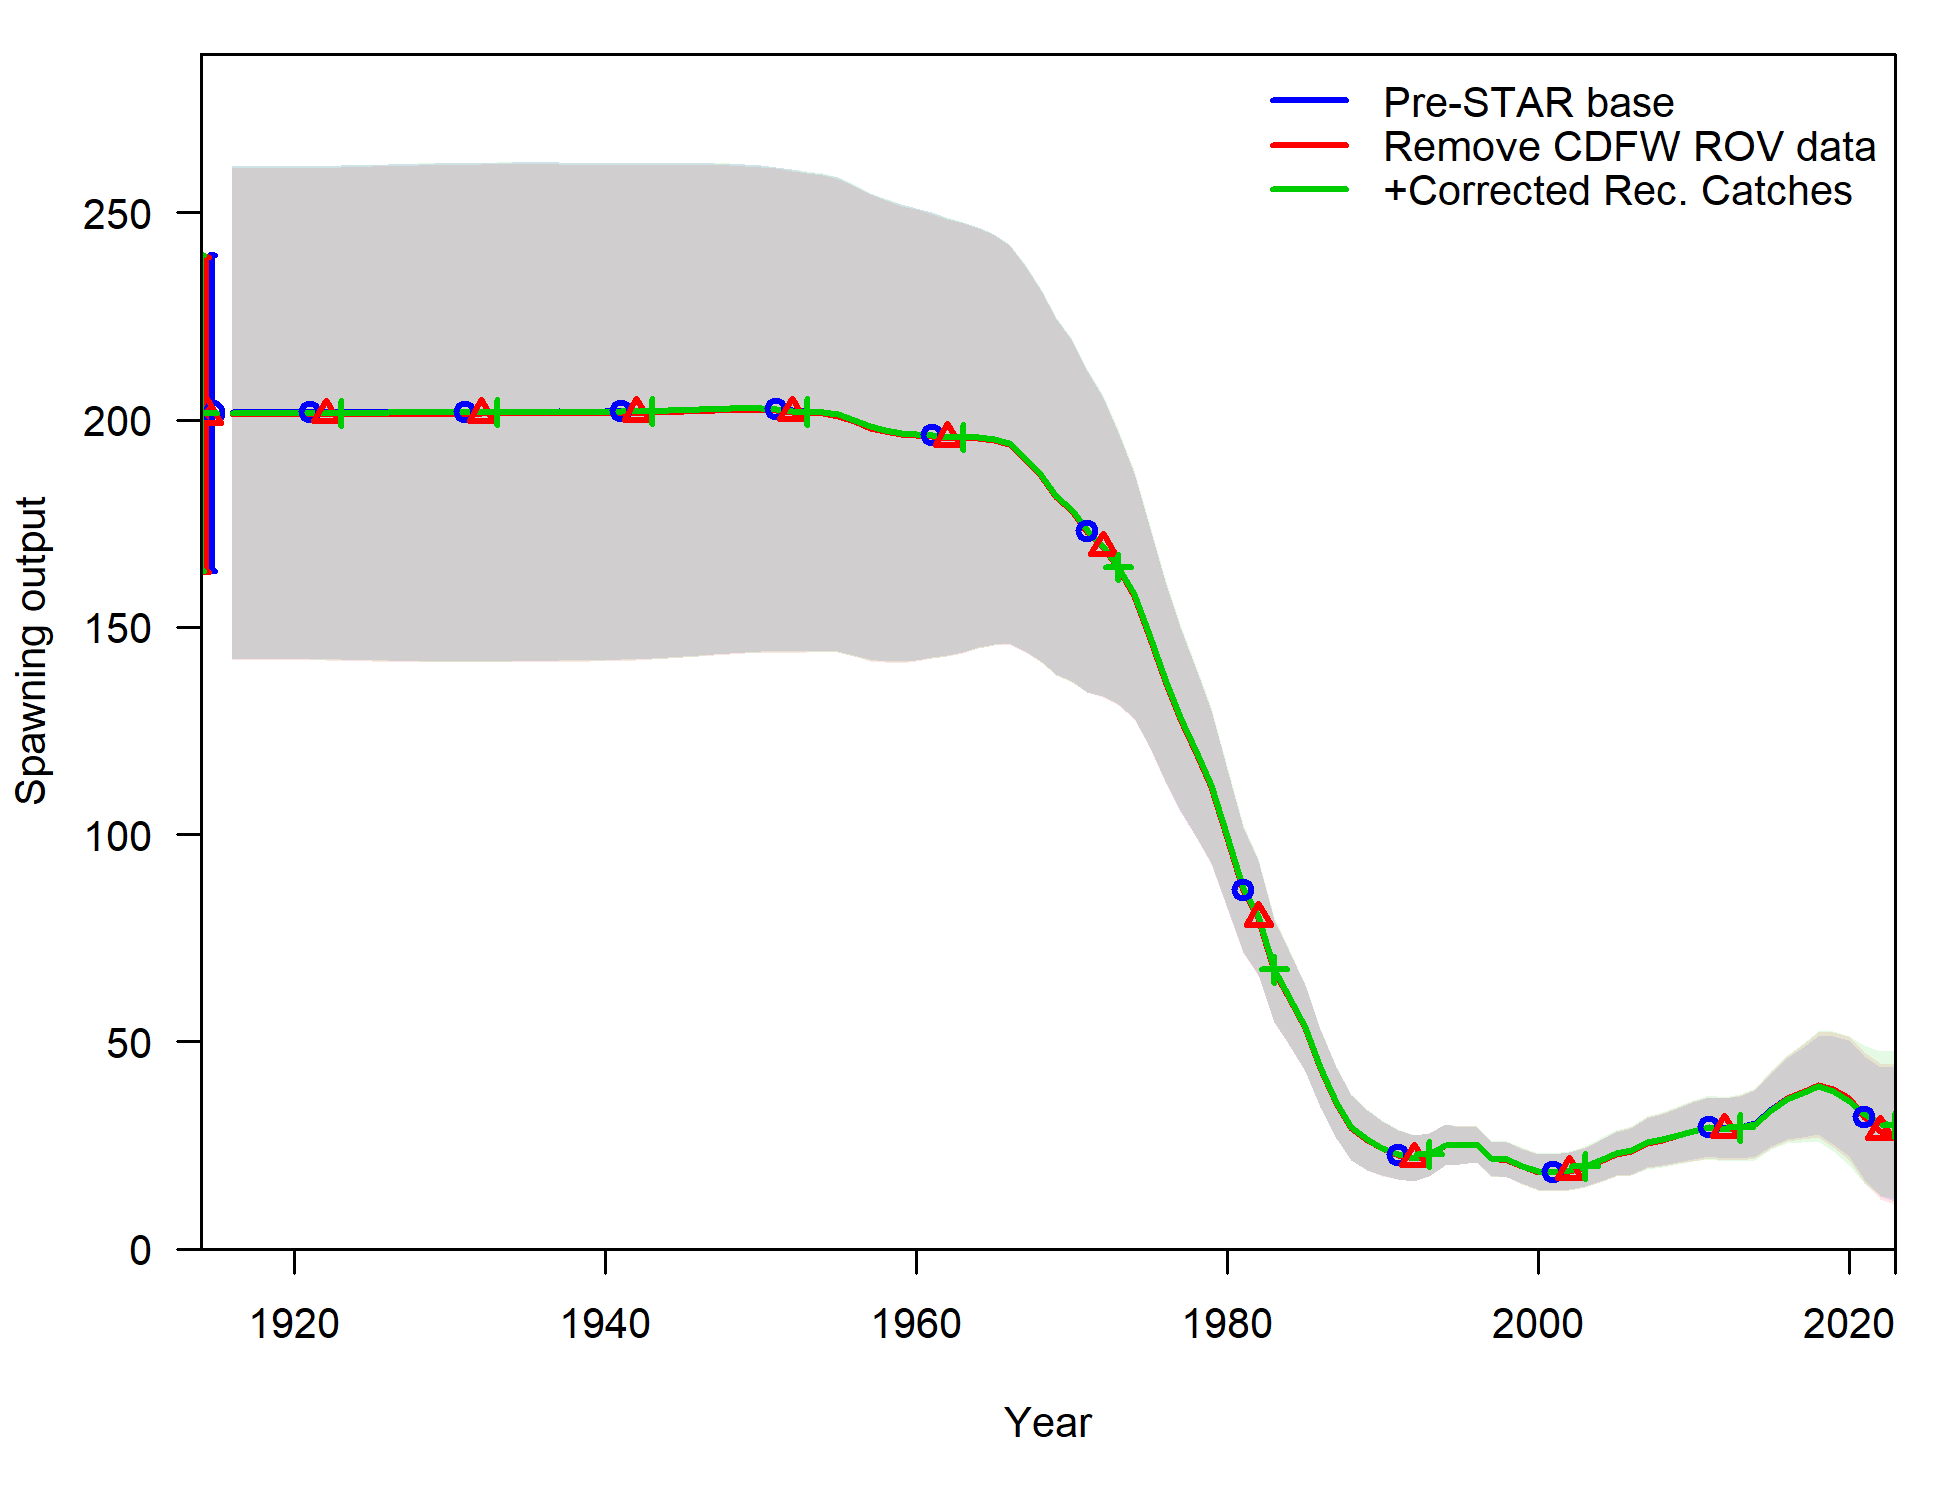
\includegraphics[width=1\textwidth,height=1\textheight]{14.3_corrected_base_compare2_spawnbio_uncertainty.png}
\caption{Estimated spawning output comparison for the sub-area model south of Point Conception between the original base model and models that remove CDFW ROV survey data, and the model with these data removed and revised 2020-21 recreational catches. The +Corrected Rec. Catches model is the revised base model.\label{fig:south-ssb}}
\end{figure}

\pagebreak

\begin{figure}
\centering
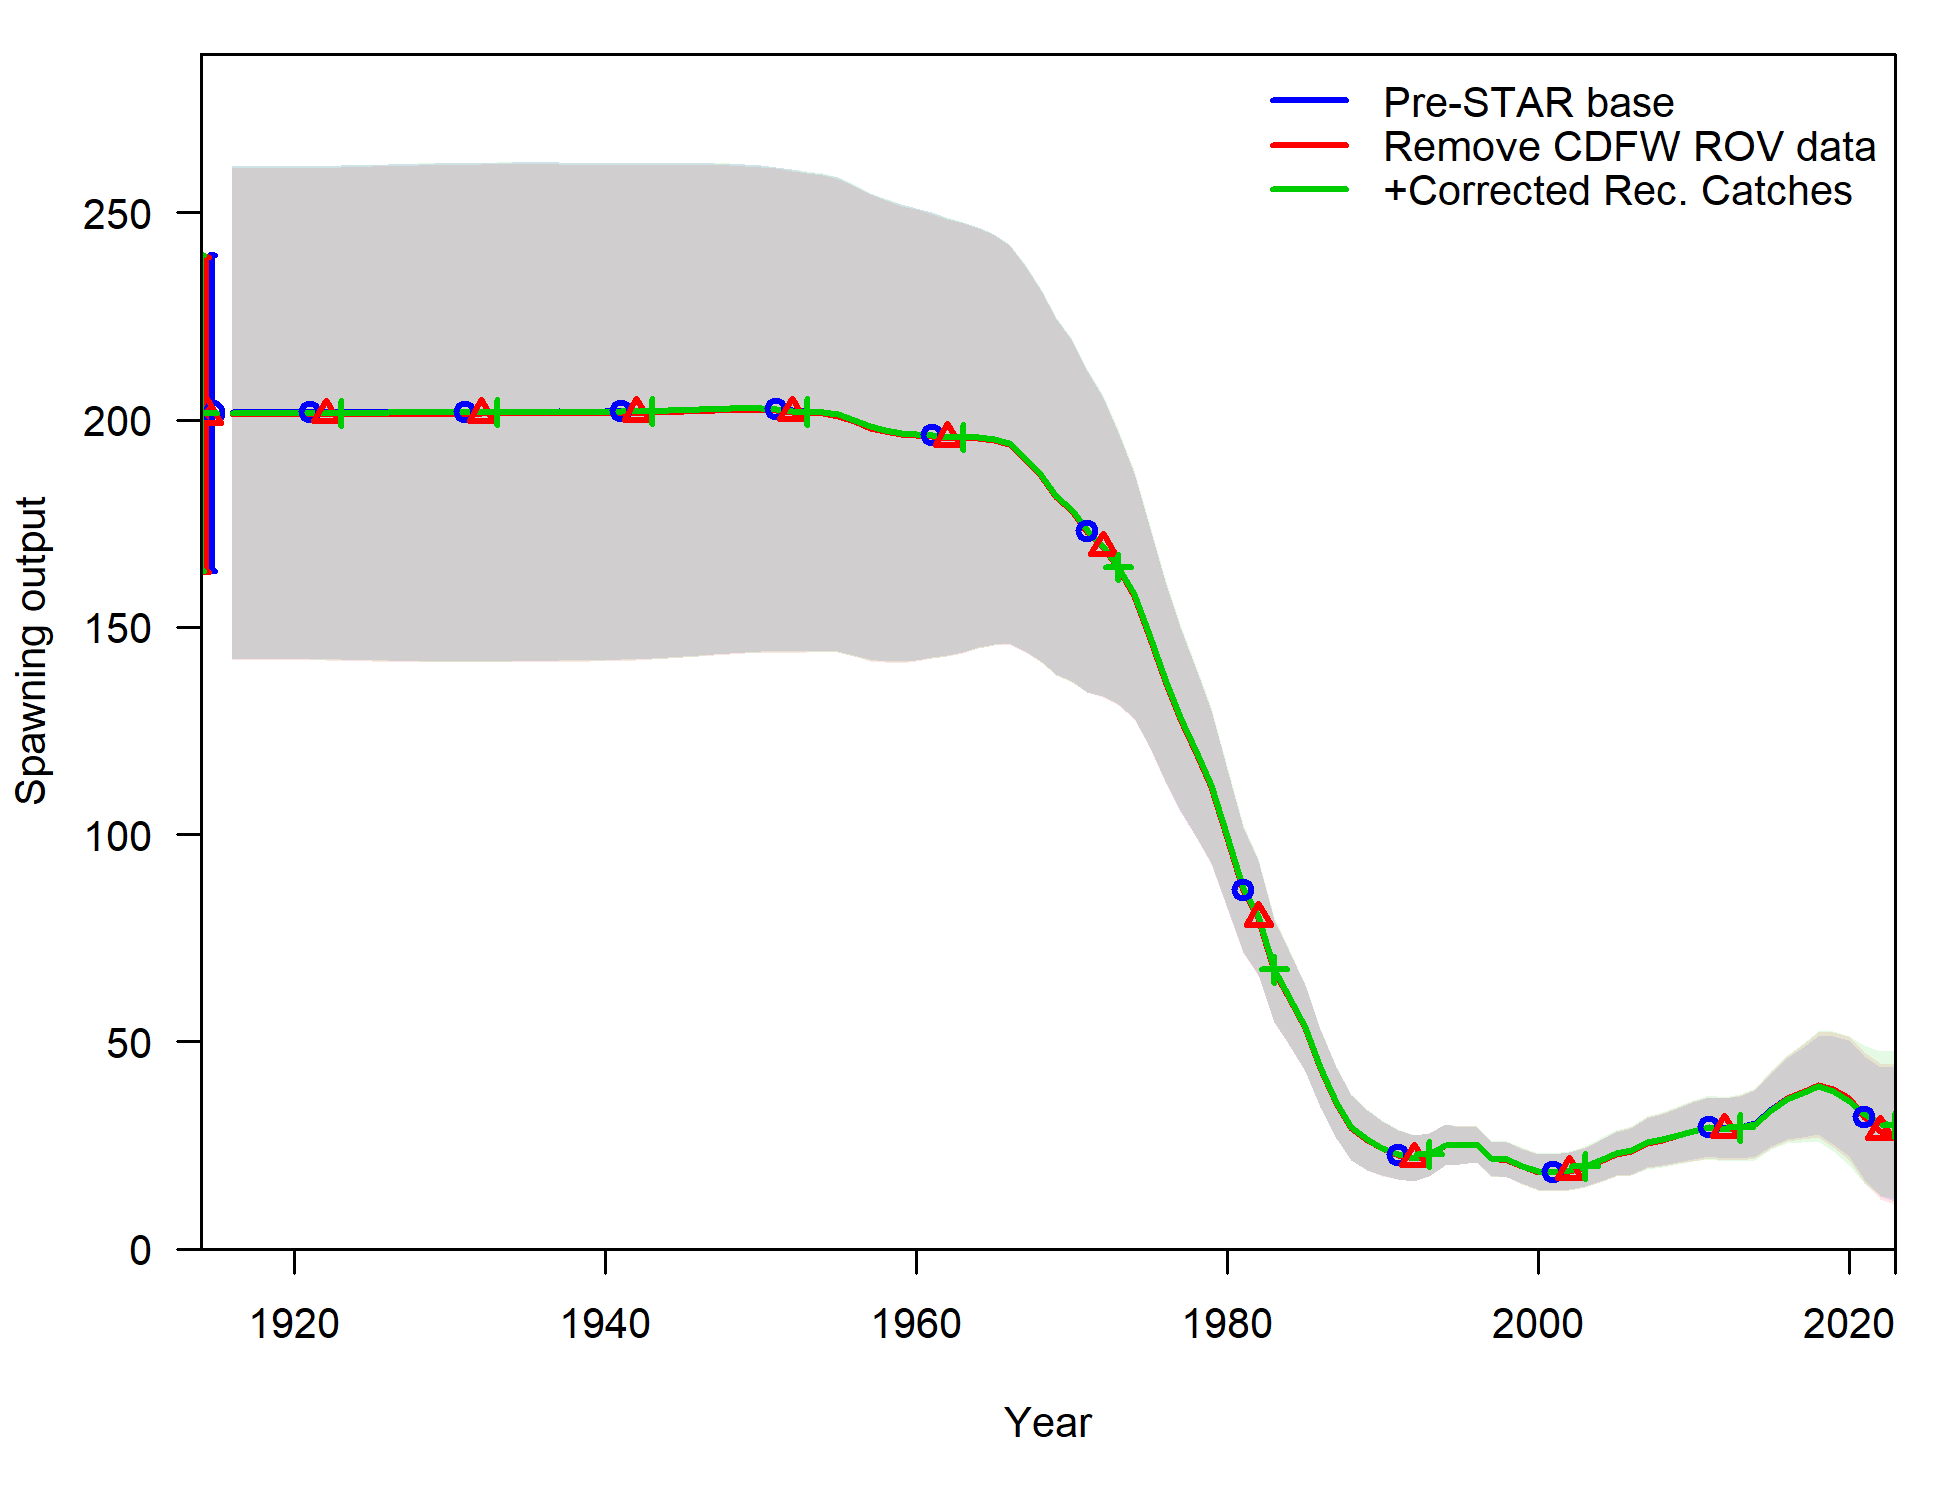
\includegraphics[width=1\textwidth,height=1\textheight]{14.3_corrected_base_compare2_spawnbio_uncertainty.png}
\caption{Estimated fraction unfished comparison for the sub-area model south of Point Conception between the original base model and models that remove CDFW ROV survey data, and the model with these data removed and revised 2020-21 recreational catches. The +Corrected Rec. Catches model is the revised base model.\label{fig:south-depl}}
\end{figure}

\pagebreak

\begin{figure}
\centering
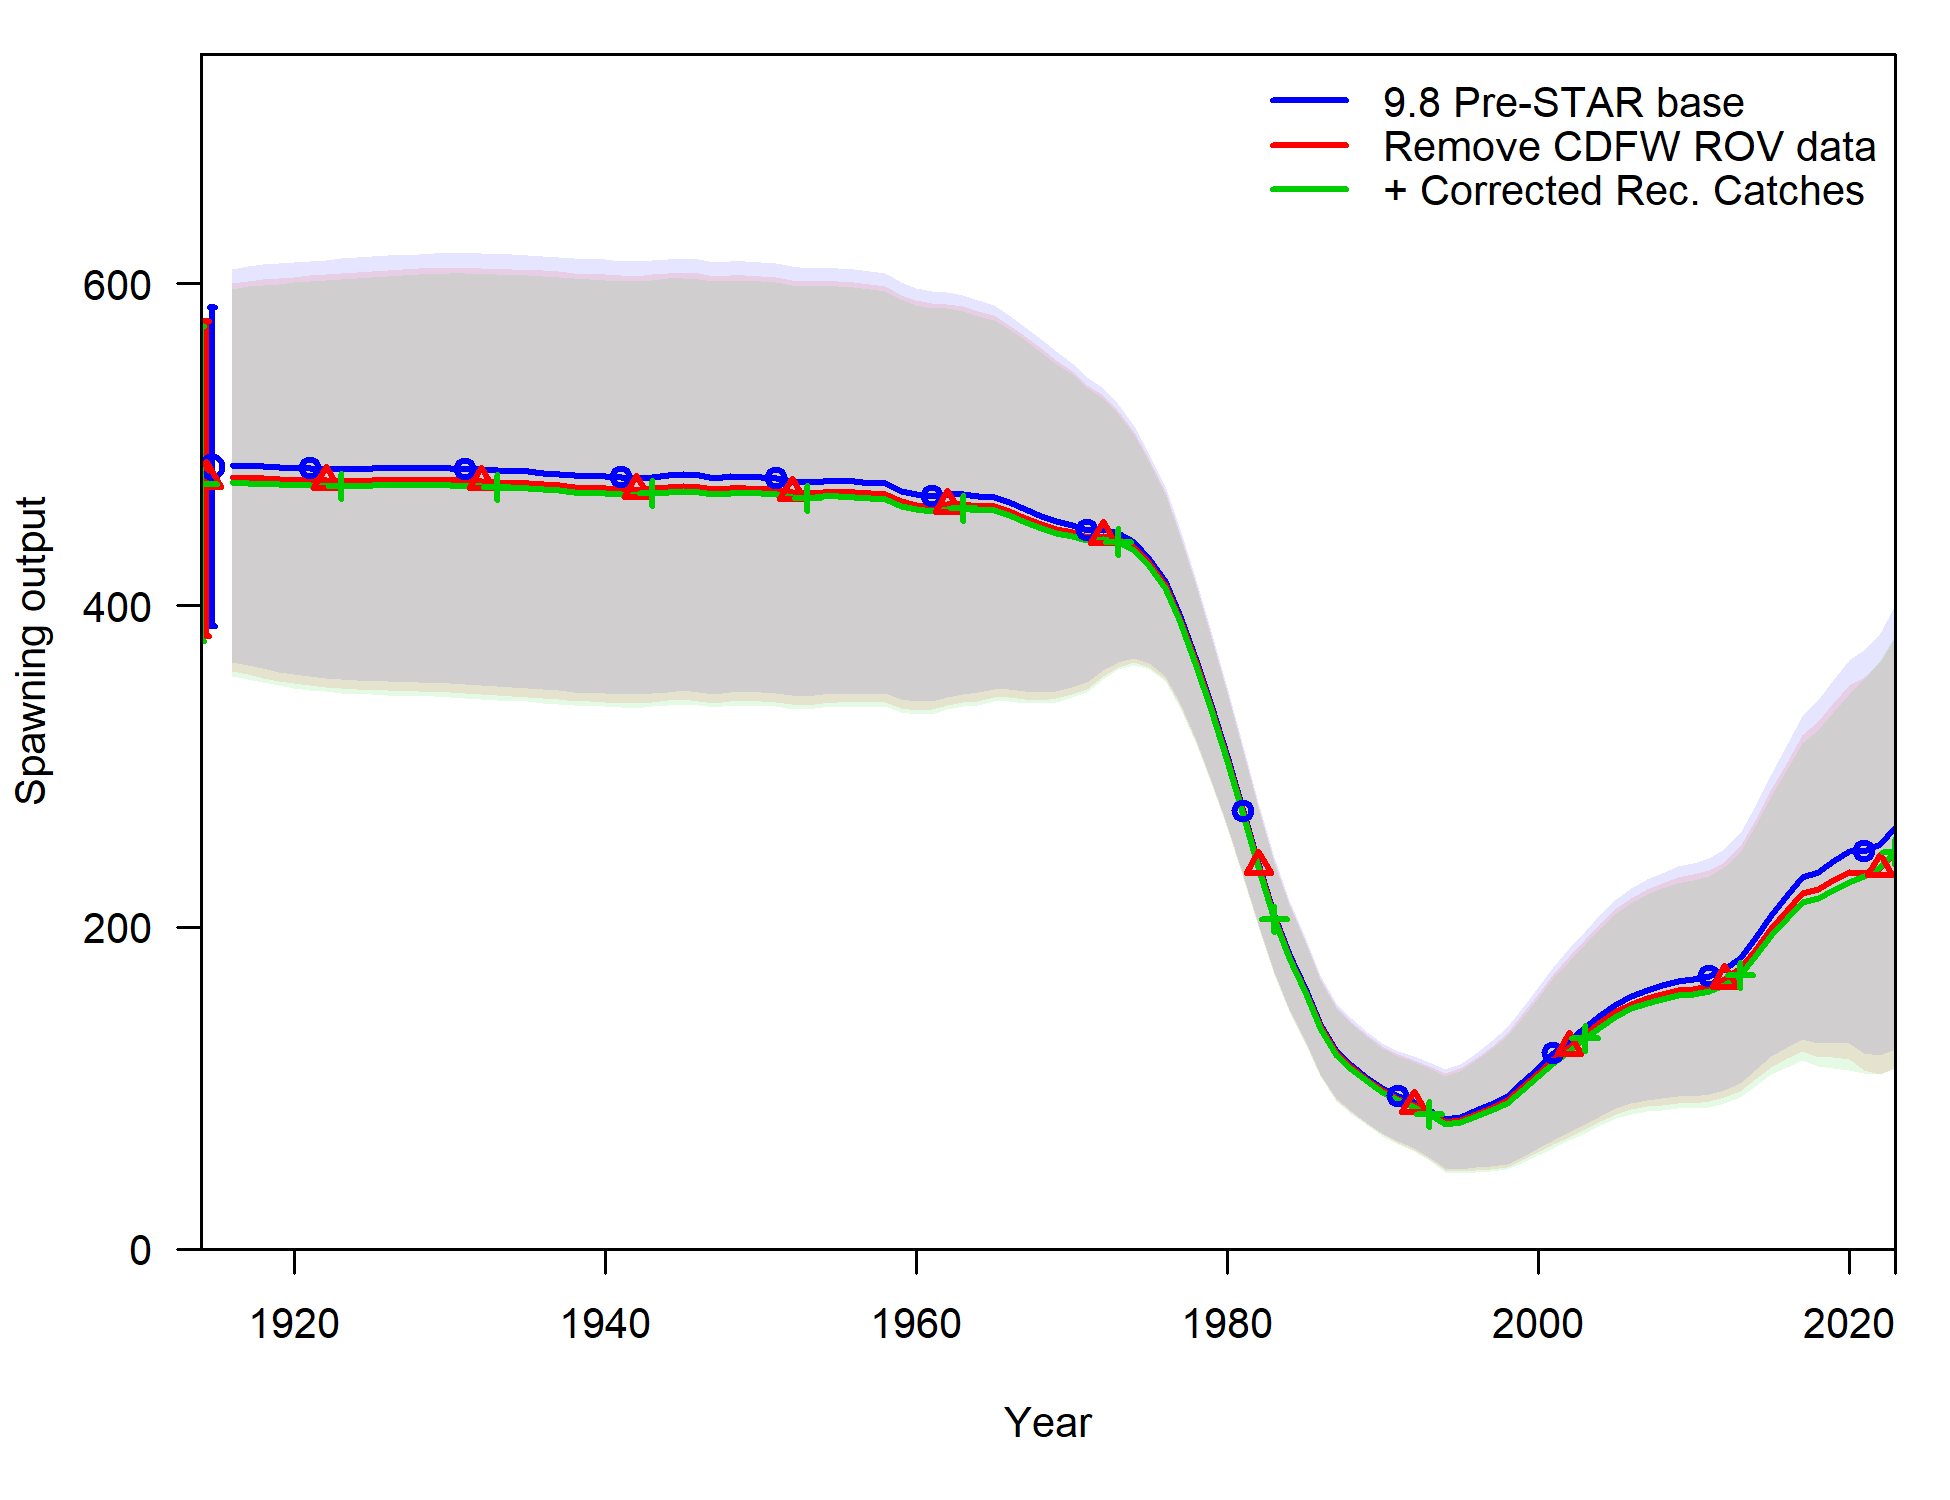
\includegraphics[width=1\textwidth,height=1\textheight]{9.10_corrected_base_compare2_spawnbio_uncertainty.png}
\caption{Estimated spawning output comparison for the sub-area model north of Point Conception between the original base model and models that remove CDFW ROV survey data, and the model with these data removed and revised 2020-21 recreational catches. The +Corrected Rec. Catches model is the revised base model.\label{fig:north-ssb}}
\end{figure}

\pagebreak

\begin{figure}
\centering
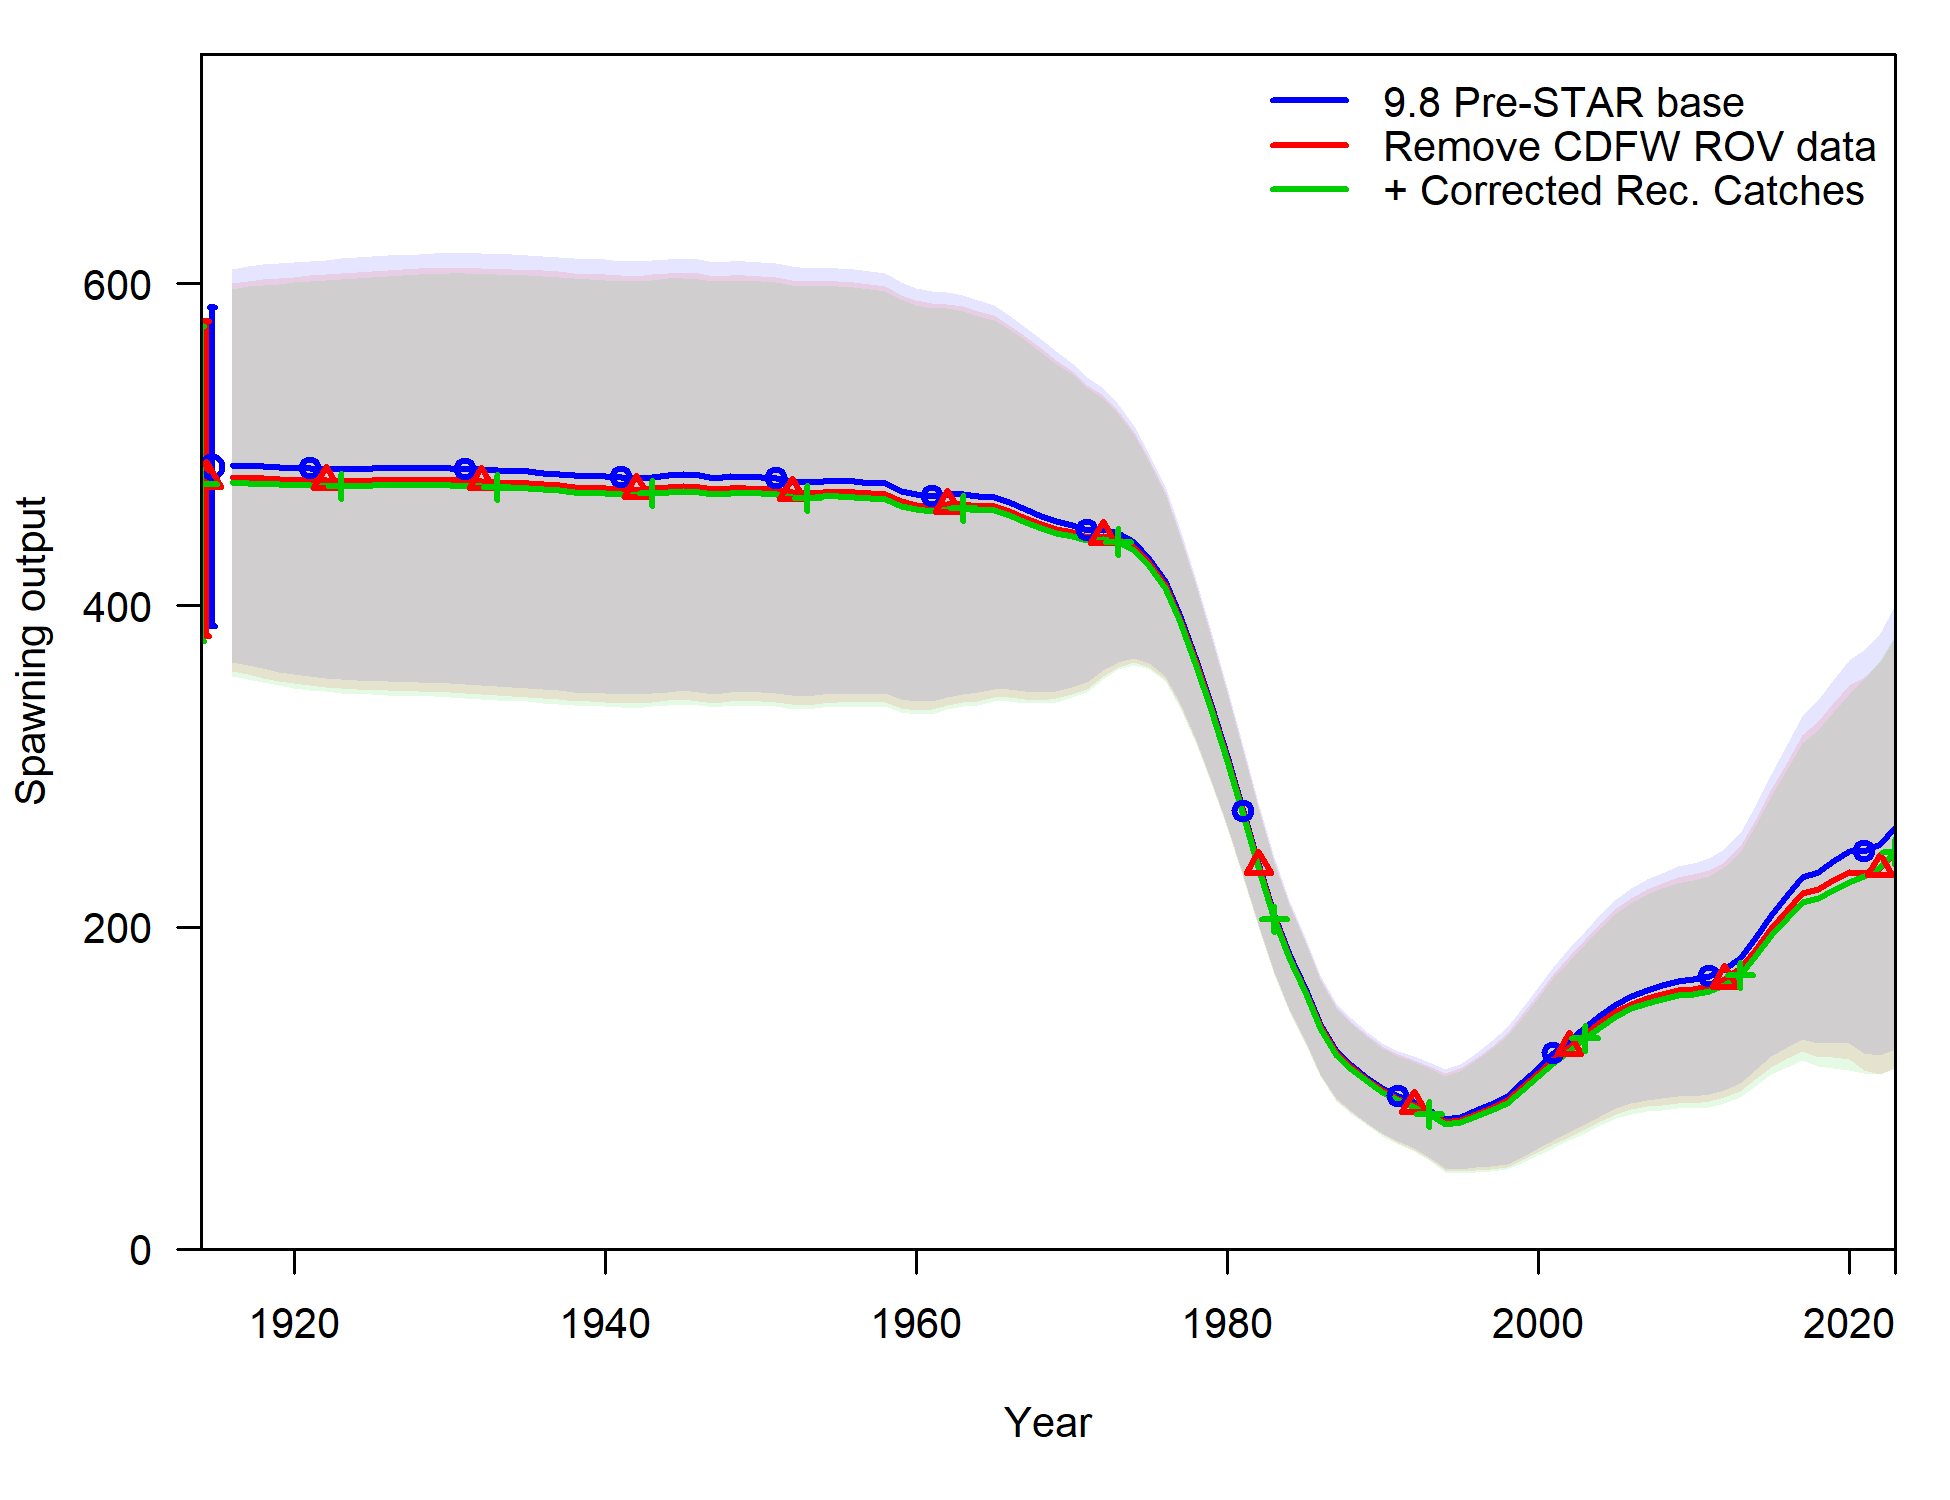
\includegraphics[width=1\textwidth,height=1\textheight]{9.10_corrected_base_compare2_spawnbio_uncertainty.png}
\caption{Estimated fraction unfished comparison for the sub-area model north of Point Conception between the original base model and models that remove CDFW ROV survey data, and the model with these data removed and revised 2020-21 recreational catches. The +Corrected Rec. Catches model is the revised base model.\label{fig:north-depl}}
\end{figure}

\pagebreak

\end{document}
